\chapter{Architecture}

% \instructions{
%     Describe the architecture of your software as covered in the SEP2 module. The main goal of this chapter is describing the \textbf{technical implementation} in a way that a new team member can start working on the product as fast as possible.
    
%     \begin{itemize}
%         \item Use an existing template as a starting point (\texttt{arc42}, \texttt{C4 model}, ...)
%         \item Focus on stable, high-level concepts rather than details
%         \item Cover different views (static, dynamic, deployment, ...)
%         \item Prefer diagrams over text (ideally UML)
%         \item Explain the reasons behind your actions: \textit{Why did we build it like this?}
%     \end{itemize}   
% }

The architecture of our application is modelled using the C4 model combined with Clean Architecture. We decide to use these models because of the lectures of SEP2 which we visit in parallel and there these models are described in detail and so we are the most familiar with these models. For our project it does not make sense to visualise all four levels of the C4 model because of the complexity we used in this project, to complete the architecture we use the Clean Architecture model to explain the dependencies.
Our application is built to use metrics which are scraped and stored by Prometheus from a Kubernetes cluster.
The functional requirements FR1 to FR11 that are tracked on GitLab have been reviewed and can all be satisfied with this architecture. 
The non-functional requirements NFR-2, NFR-3, NFR-4, are possible to satisfy with the technologies shown in the section Clean Architecture.
The application will be built inside a container to satisfy NFR-5.

\section{Roles}
The role of the architect is split up. We work according to the architecture agent model, where we have two architects.
Jan is responsible for Kubernetes, Prometheus, CI/CD, i.e. the architecture at large
and Pascal is responsible for the architecture of our web application, which libraries are used and how we connect the different components, i.e. the "architecture at small". We decided to choose the model with two main architects because of the two project parts we need to handle and so there is each person from each part to discuss the interfaces and the perfect architecture over all project parts.

\section{System Architecture according to C4 model}
\begin{figure}[H]
  \centering
  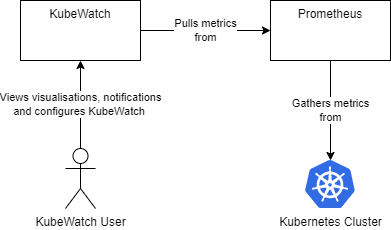
\includegraphics[height=5cm]{resources/System_context_diagram.png}
  \caption{System context diagram}
  \label{fig:system-context-diagram}
\end{figure}

\begin{figure}[H]
  \centering
  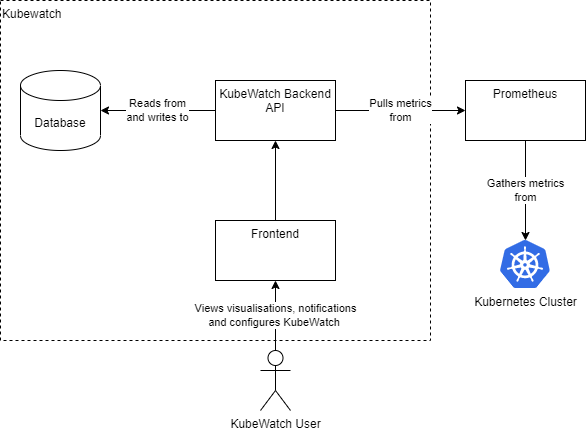
\includegraphics[height=8cm]{resources/Container_diagram.png}
  \caption{Container diagram}
  \label{fig:container-diagram}
\end{figure}

\section{CI/CD Pipeline Architecture}

\begin{figure}[H]
  \centering
  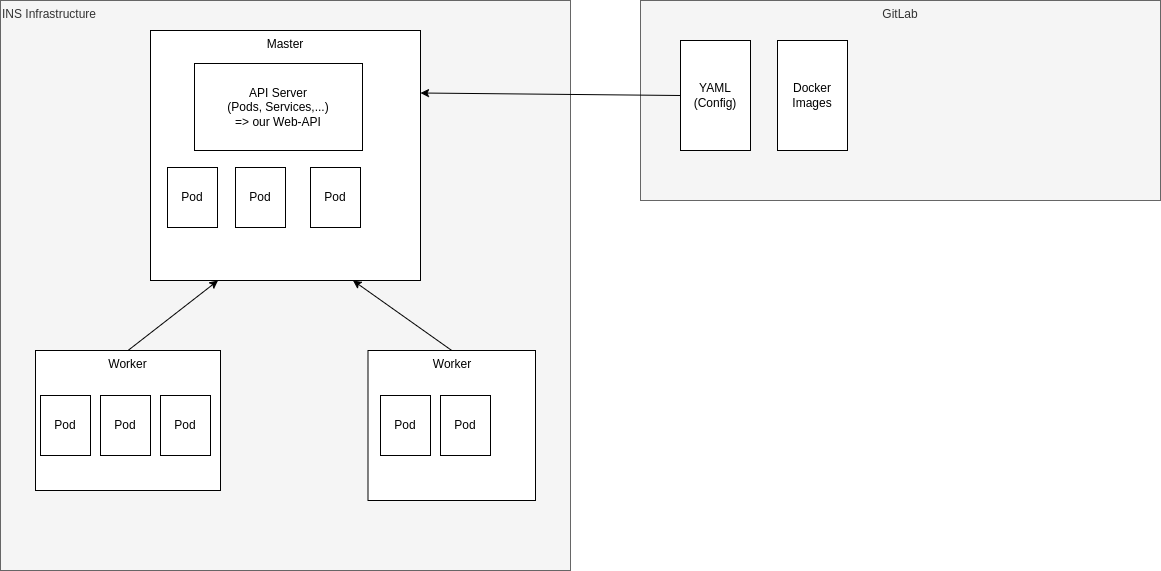
\includegraphics[height=7.3cm]{resources/architecture.png}
  \caption{KubeWatch CI/CD Pipeline architecture}
  \label{fig:architecture}
\end{figure}

\begin{table}[H]
  \begin{tabular*}{\textwidth}{p{3.5cm} | p{9cm}}
    \textbf{Master:}
      & Each Kubernetes cluster contains at least one master node which runs the Kubernetes control plane. These control plane consists of an API server, scheduler, controller manager, etc. \bigskip \\
    \textbf{Worker/Node:}
      & Each cluster includes at least one worker node, this node runs containerized applications. Each worker node host \textit{Pods}. \bigskip \\
    \textbf{Pod:}
      & A pod is a component of the application workload. \\
  \end{tabular*}
  \caption{K8s elements explained}
  \label{tab:k8s-elements-explained}
\end{table}

\section{Web App Clean Architecture}
\begin{figure}[H]
  \centering
  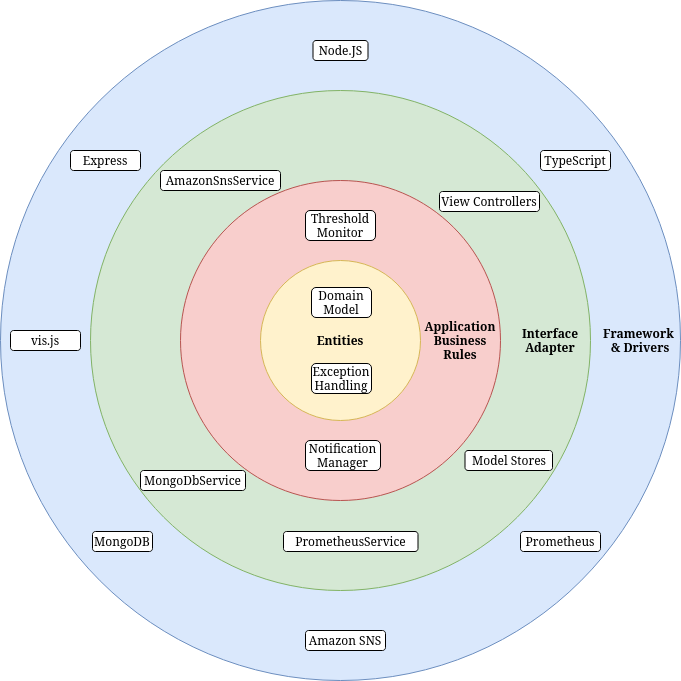
\includegraphics[height=14cm]{resources/clean_architecture.drawio.png}
  \caption{Web app clean architecture}
  \label{fig:web-app-architecture}
\end{figure}

\begin{table}[H]
  \begin{tabular*}{\textwidth}{p{3cm} | p{11cm}}
    \textbf{Entities:}
      & These are components shared by the whole system and is contained in the \textit{/model} directory. This includes the classes from the domain model as well as exception handling. Additionally the model store interfaces are contained here, allowing implementation from the Interface Adapter layer. \bigskip \\
    \textbf{Application Business Rules:}
      & This layer contains our business logic and is contained in the \textit{/domain} directory. \bigskip \\
    \textbf{Interface Adapter:}
      & This is the place for logic to attach to our external dependecies like Prometheus and MongoDB and is contained in the \textit{/services} and \textit{/view-controllers} directories. The implementations of the model store interfaces are also stored here. \bigskip \\
    \textbf{Framework \& Drivers:}
      & These are the major frameworks and dependencies powering our application. \\
  \end{tabular*}
  \caption{Clean-Architecture layers explained}
  \label{tab:clean-architecture-layers-explained}
\end{table}

\section{Wireframe}

To visualise the application draft we decide to use a wireframe because it makes a lot of sense with the web application \textit{KubeWatch} we programme in this project. So for a detailed overview, we can just click through the wireframe to get an impression. The complete wireframe can be found as a PDF\footnote{\url{https://gitlab.ost.ch/SEProj/2022-FS/g03-kubewatch/kubewatch/-/blob/main/Documentation/appendix/wireframe_kubewatch.drawio.pdf}} and HTML page\footnote{\url{https://gitlab.ost.ch/SEProj/2022-FS/g03-kubewatch/kubewatch/-/blob/main/Documentation/appendix/wireframe_kubewatch.drawio.html}} in the appendix directory.
The HTML page is interactive.
